\section{Introduction}

Information fusion only works after one has decided what the pieces of evidence mean. In many sensor and multi-view settings this decision is implicit: a feature column, a modality, or a calibrated channel carries the same identity wherever it appears \cite{castanedo2013datafusion,lahat2015multimodal,baltrusaitis2019multimodal,zhao2017multiview}. Federated learning (FL) inherits the same assumption when the server combines local information without seeing raw data \cite{mcmahan2017fedavg,yang2019federated,kairouz2021advances}. Quantum readout is a useful stress case, not the only target domain: local evidence consists of finite-shot estimates of quantum observables, and a coordinate is a measurement choice rather than a disposable feature index \cite{huang2020classicalshadows,hadfield2022locallybiased,bu2024pauli}.

In classical FL, a vector update usually has a shared meaning because all clients use the same parameterization, feature space, or classifier head \cite{mcmahan2017fedavg,kairouz2021advances}. In heterogeneous source fusion this assumption can fail when views, sensors, measurement coordinates, or local feature orders differ across clients, a setting closely related to incomplete multi-view learning, missing-modality fusion, and multimodal FL \cite{havaei2016hemis,tang2024incomplete,cai2024projected,lin2023federatedmultimodal}. Quantum readout makes the failure especially explicit. Client \(i\) may report expectations of one subset of Pauli strings, client \(j\) another subset, and their local coordinate orders may be arbitrary \cite{havlicek2019supervised,schuld2019feature,huang2020classicalshadows}. Even if both clients upload class prototypes of the same length, coordinate \(a\) of one prototype may correspond to a different observable than coordinate \(a\) of another. Direct averaging is then not a well-defined semantic operation.

We study this failure mode as incomplete-view information fusion over heterogeneous source coordinates, using quantum measurement as the motivating case. The object to define is not merely a prototype, but a \emph{comparability protocol}: source identities, missingness, public anchors, sketches, and aggregation rules that make client statistics commensurate before server-side fusion. Schema binding is therefore not bookkeeping. It is the step that gives a distributed fusion rule a semantic domain. Fig.~\ref{fig:if-framework} gives the overall picture. Our instantiation, \method, combines schema adapters, random Fourier feature (RFF) kernel sketches, and coverage-aware observable aggregation, building on prototype FL, random features, and kernel mean embeddings while changing the comparability assumption under which they are used \cite{tan2022fedproto,rahimi2007random,smola2007hilbert,gretton2012mmd}. The novelty is protocol-level: value-mask vectors, prototypes, and random sketches are familiar tools, but here they are tied to an explicit rule for when heterogeneous coordinates are semantically comparable. We also include a mask-aware high-order outer-product extension, \hopmethod, for cases where covariance or cross-source interactions carry the class signal.



\begin{figure*}[t]
    \centering
    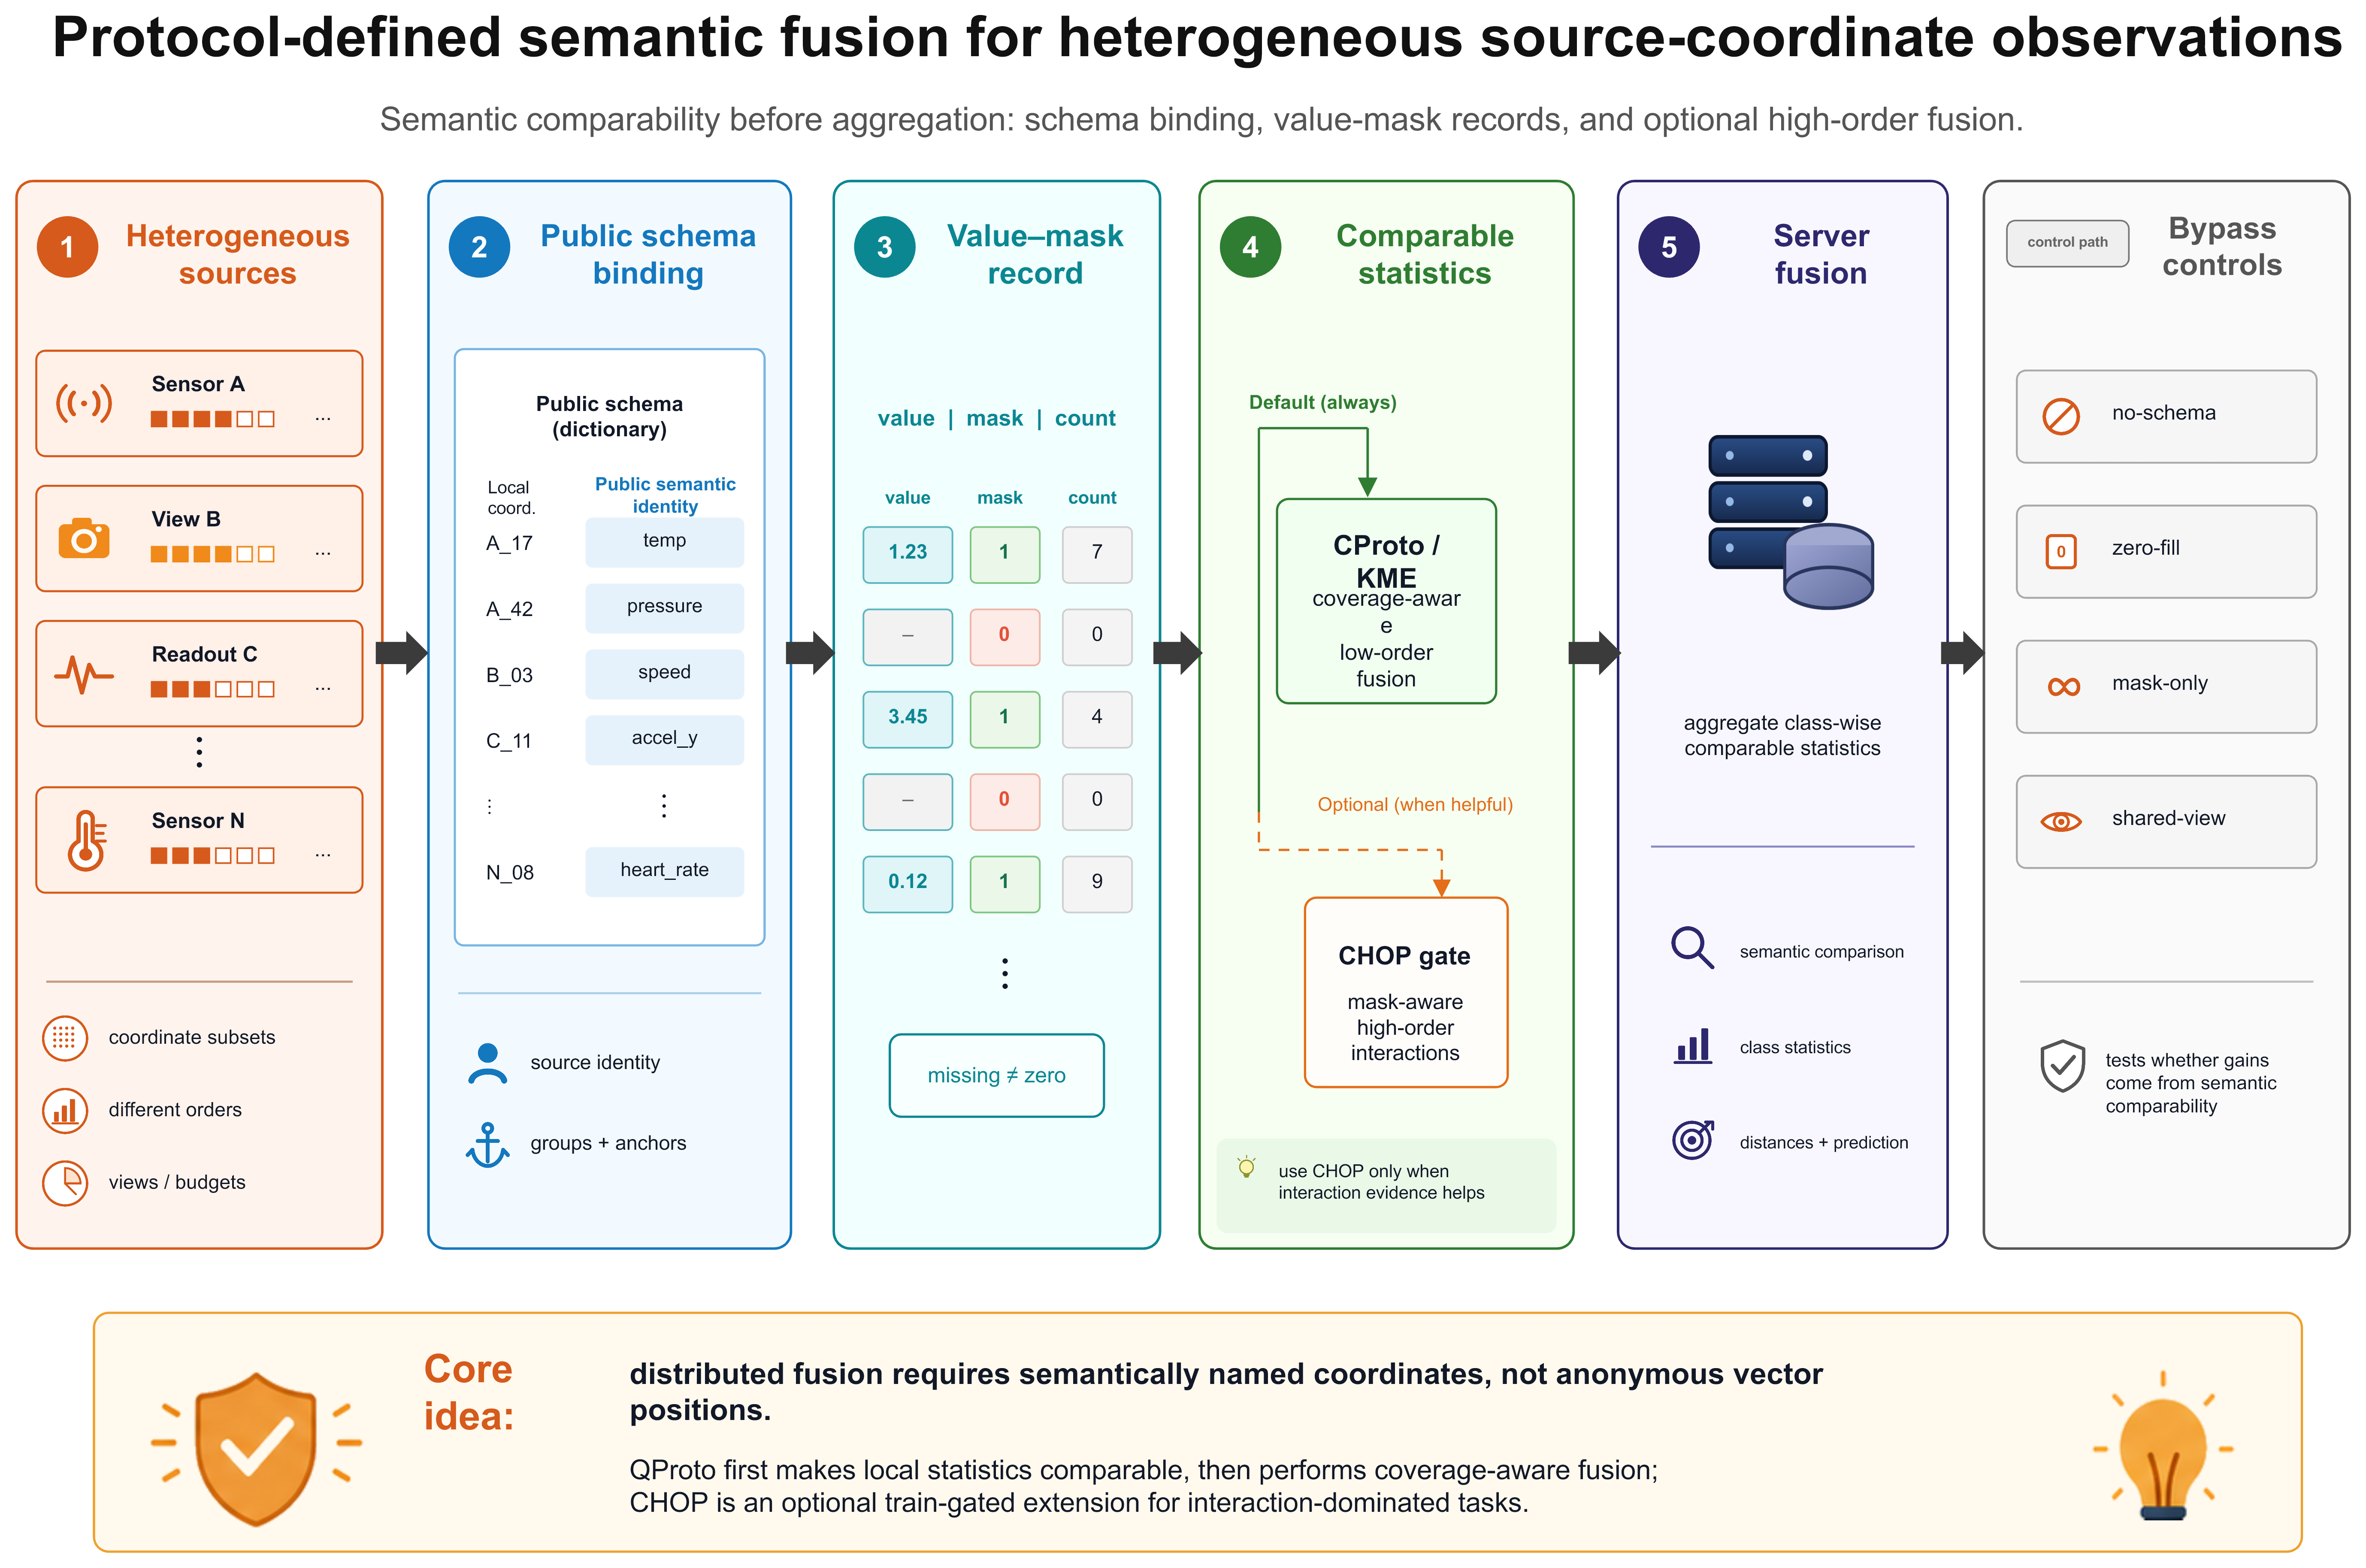
\includegraphics[width=\textwidth]{figures/fig1_semantic_fusion_redrawn_v45_cropped.png}
    \caption{Protocol-defined semantic fusion for heterogeneous source-coordinate observations. Local sources may expose different coordinate subsets, orders, views, noise levels, or measurement budgets. \method\ first binds local coordinates to public semantic identities, then maps observations into value-mask records with coverage counts so that missing measurements are not confused with measured near-zero values. The default path performs low-order coverage-aware CProto/KME fusion, while CHOP is a train-gated high-order extension used only when interaction evidence helps. The bypass controls test whether gains come from semantic comparability rather than anonymous vector averaging.}
    \label{fig:if-framework}
\end{figure*}



Operationally, a client first converts its local readout into a public value-and-mask representation. Values store observed expectation estimates; masks say which protocol coordinates were actually measured. This small distinction is essential because a missing observable and an observed expectation near zero should not be fused as the same event. The default server statistic is low-order: either a finite-dimensional kernel mean sketch or a coverage-aware observable prototype that keeps value sums and coverage counts for each public coordinate. When second-order structure is needed, projected mask-aware outer products add a compressed high-order statistic normalized by the visible coordinate subset. We also implement finite-shot variance shrinkage, but it acts as a reliability hook rather than the main contribution.

The experiments are organized to test one question: what breaks when schema, mask, and coverage are not explicit parts of the fusion rule? In MNIST-4, Fashion-MNIST-4, and CIFAR-4 feature experiments with heterogeneous readout, the no-schema, wrong-schema, forced-canonical, FedAvg, and FedProx controls expose the cost of aggregating statistics whose coordinates are not comparable. In the full-class MNIST-10, Fashion-10, and CIFAR-10 evaluations, the coverage-aware \hopmethod\ variant reaches 0.744, 0.662, and 0.454 accuracy, while the IF-style controls rule out explanations based only on schema metadata, zero-imputation, or shared-observable intersection. The non-quantum checks use the same abstraction on UCI HAR smartphone sensors, UCI Multiple Features, MHEALTH/PAMAP2 wearables, Hydraulic Systems condition monitoring, and WDBC biomedical features. CProto reaches 0.753 on UCI HAR under the same payload where zero-fill RFF and shared-view RFF obtain 0.344 and 0.391. On Multiple Features, group-balanced CProto matches view-wise late fusion at 0.949 and reaches 0.876 under a strict compressed payload; random-key low-order compression is also strong there, so the dataset supports schema-aware low-order fusion rather than a universal key-selection advantage. On subject-held-out MHEALTH, adaptive CHOP reaches 0.878 at the same 13,876-byte payload where low-order CProto obtains 0.860; HeMIS reaches 0.889 and is treated as a centralized trainable boundary. On Hydraulic Systems, compact equal-byte CProto/CHOP reach 0.973/0.977 versus 0.833 for shared-view RFF, while HeMIS reaches 0.997. These comparisons delimit the high-order claim. On many image, sensor, multi-view, and biomedical tasks, semantic coverage-aware fusion is the main gain and HOP is not automatically helpful. For interaction-heavy tasks it becomes important: CHOP reaches 0.732 versus 0.358 for matched low-order CProto in the main covariance-sensing benchmark; supplementary PennyLane high-order readouts improve from 0.422 to 0.550 with mask-aware HOP; and a synthetic covariance benchmark reaches 0.808 versus 0.467 for the low-order variant.

The contributions follow the information-fusion logic of the problem. First, we formulate semantic coordinate comparability as a prerequisite for distributed prototype fusion. Second, we introduce the \method\ value-mask and coverage-count backbone for low-order kernel or source prototypes, including source-group normalization when view dimensionalities differ. Third, we add mask-aware \hopmethod/CHOP as a conditional extension for covariance- or interaction-dominated tasks, with a train-calibrated fallback to low-order CProto. Fourth, we give failure-mode and consistency analyses showing why schema mismatch creates non-vanishing semantic bias. The empirical package is deliberately broad: heterogeneous quantum-readout evaluations, real UCI HAR/MFeat/MHEALTH/PAMAP2/Hydraulic/WDBC missing-view fusion, Qiskit Aer/PennyLane compatibility checks, and covariance-dominated stress tests, all with schema, imputation, deep missing-view, FL/QFL, and equal-byte controls.





